\chapter{Metode}
\label{cap:metode}

Acest capitol prezintă metodele de machine learning utilizate pentru predicția răspunsului la medicamente din expresia genică. Am implementat și comparat trei abordări complementare: Random Forest, XGBoost și Rețele Neuronale.

\section{Formularea Problemei}
\label{sec:formulare}

Predicția răspunsului la medicamente poate fi formalizată ca o problemă de regresie:

\begin{equation}
y = f(\mathbf{x}_{\text{gene}}, d) + \epsilon
\end{equation}

unde:
\begin{itemize}
    \item $y \in \mathbb{R}$ este răspunsul la medicament (IC50 sau AUC)
    \item $\mathbf{x}_{\text{gene}} \in \mathbb{R}^{5000}$ este vectorul de expresie genică
    \item $d \in \{1, 2, ..., 200\}$ este ID-ul medicamentului
    \item $f$ este funcția de predicție pe care dorim să o învățăm
    \item $\epsilon$ este zgomotul aleatoriu (variabilitate experimentală, factori neobservați)
\end{itemize}

Obiectivul este să învățăm funcția $\hat{f}$ care aproximează cât mai bine $f$ pe baza datelor de antrenare $\mathcal{D} = \{(\mathbf{x}_i, d_i, y_i)\}_{i=1}^{N}$.

\subsection{Pan-Drug vs Per-Drug Modeling}
\label{subsec:pan_vs_per}

Există două abordări principale pentru predicția răspunsului:

\begin{itemize}
    \item \textbf{Per-drug modeling}: Antrenarea unui model separat pentru fiecare medicament. Avantaj: model specializat pentru fiecare medicament. Dezavantaj: necesită multe date per medicament și nu poate generaliza la medicamente noi.

    \item \textbf{Pan-drug modeling}: Antrenarea unui singur model pentru toate medicamentele, cu ID-ul medicamentului ca un feature suplimentar. Avantaj: poate învăța pattern-uri generale și poate face predicții pentru medicamente noi. Dezavantaj: modelul trebuie să învețe să diferențieze între medicamente.
\end{itemize}

În această lucrare am adoptat abordarea \textbf{pan-drug}, permițând modelului să învețe pattern-uri generale de răspuns la medicamente și să beneficieze de transfer learning între medicamente similare.

\section{Random Forest}
\label{sec:random_forest}

Random Forest \cite{breiman2001random} este un algoritm de ensemble learning bazat pe decision trees (arbori de decizie).

\subsection{Principiul Algoritmului}
\label{subsec:rf_principiu}

Un decision tree împarte recursiv spațiul de features, creând reguli de forma:
\begin{center}
\textit{``Dacă gene\_X > threshold, atunci..."}
\end{center}

Random Forest combină predicțiile a $T$ arbori independenți:

\begin{equation}
\hat{y} = \frac{1}{T} \sum_{t=1}^{T} h_t(\mathbf{x})
\end{equation}

unde $h_t$ este predicția arborelui $t$.

\subsection{Diversitatea Arborilor}
\label{subsec:rf_diversity}

Pentru a asigura că arborii sunt diferiți și complementari:

\begin{itemize}
    \item \textbf{Bagging (Bootstrap Aggregating)}: Fiecare arbore este antrenat pe un subset aleatoriu (cu înlocuire) din datele de antrenare.

    \item \textbf{Feature randomness}: La fiecare split, doar un subset aleatoriu de $\sqrt{p}$ features este considerat (unde $p$ = 5,001 în cazul nostru).
\end{itemize}

Această randomizare reduce corelația între arbori, îmbunătățind generalizarea.

\subsection{Hiperparametri}
\label{subsec:rf_params}

Principalii hiperparametri utilizați:

\begin{table}[h]
\centering
\caption{Hiperparametri Random Forest}
\label{tab:rf_params}
\begin{tabular}{lrl}
\toprule
\textbf{Parametru} & \textbf{Valoare} & \textbf{Descriere} \\
\midrule
n\_estimators & 500 & Numărul de arbori \\
max\_depth & 20 & Adâncimea maximă a arborilor \\
min\_samples\_split & 10 & Număr minim de sample-uri pentru split \\
max\_features & sqrt & Număr de features per split ($\sqrt{5001} \approx 71$) \\
\bottomrule
\end{tabular}
\end{table}

\subsection{Avantaje și Dezavantaje}
\label{subsec:rf_pros_cons}

\textbf{Avantaje}:
\begin{itemize}
    \item Robust la overfitting (prin averaging)
    \item Poate captura interacțiuni non-liniare complexe
    \item Furnizează feature importance (ce gene sunt importante)
    \item Nu necesită normalizare
\end{itemize}

\textbf{Dezavantaje}:
\begin{itemize}
    \item Poate fi mai puțin performant decât gradient boosting pe date tabulare
    \item Memorie mare (păstrează toți arborii)
\end{itemize}

\section{XGBoost}
\label{sec:xgboost}

XGBoost (eXtreme Gradient Boosting) \cite{chen2016xgboost} este un algoritm de gradient boosting optimizat pentru performanță și acuratețe.

\subsection{Gradient Boosting}
\label{subsec:gradient_boosting}

Spre deosebire de Random Forest (unde arborii sunt independenți), gradient boosting construiește arbori secvenițial, fiecare corectând erorile precedentului.

Algoritmul:
\begin{enumerate}
    \item Inițializare: $F_0(\mathbf{x}) = \bar{y}$ (media valorilor țintă)
    \item Pentru $m = 1$ până la $M$:
    \begin{enumerate}
        \item Calcularea reziduurilor: $r_i = y_i - F_{m-1}(\mathbf{x}_i)$
        \item Antrenarea unui arbore $h_m$ pentru a prezice reziduurile
        \item Actualizarea modelului: $F_m(\mathbf{x}) = F_{m-1}(\mathbf{x}) + \eta \cdot h_m(\mathbf{x})$
    \end{enumerate}
    \item Predicția finală: $\hat{y} = F_M(\mathbf{x})$
\end{enumerate}

unde $\eta$ este learning rate (rata de învățare).

\subsection{Regularizare}
\label{subsec:xgb_regularizare}

XGBoost adaugă termeni de regularizare la funcția obiectiv pentru a preveni overfitting:

\begin{equation}
\mathcal{L} = \sum_{i=1}^{N} l(y_i, \hat{y}_i) + \sum_{t=1}^{T} \Omega(h_t)
\end{equation}

unde:
\begin{itemize}
    \item $l$ este funcția de loss (MSE în cazul nostru)
    \item $\Omega(h_t)$ penalizează complexitatea arborelui $t$ (număr de frunze, magnitudinea ponderilor)
\end{itemize}

\subsection{Early Stopping}
\label{subsec:early_stopping}

XGBoost suportă early stopping: antrenarea se oprește dacă performanța pe setul de validare nu se îmbunătățește după un număr fix de iterații. Aceasta previne overfitting și reduce timpul de antrenare.

\subsection{Hiperparametri}
\label{subsec:xgb_params}

Principalii hiperparametri utilizați:

\begin{table}[h]
\centering
\caption{Hiperparametri XGBoost}
\label{tab:xgb_params}
\begin{tabular}{lrl}
\toprule
\textbf{Parametru} & \textbf{Valoare} & \textbf{Descriere} \\
\midrule
learning\_rate & 0.05 & Rata de învățare $\eta$ \\
n\_estimators & 1000 & Număr maxim de arbori \\
max\_depth & 6 & Adâncimea maximă a arborilor \\
early\_stopping & 50 & Stop după 50 iterații fără îmbunătățire \\
subsample & 0.8 & Fracția de sample-uri per arbore \\
colsample\_bytree & 0.8 & Fracția de features per arbore \\
\bottomrule
\end{tabular}
\end{table}

\subsection{Avantaje și Dezavantaje}
\label{subsec:xgb_pros_cons}

\textbf{Avantaje}:
\begin{itemize}
    \item Adesea cel mai performant algoritm pe date tabulare
    \item Regularizare automată previne overfitting
    \item Early stopping reduce timpul de antrenare
    \item Poate utiliza GPU pentru accelerare
\end{itemize}

\textbf{Dezavantaje}:
\begin{itemize}
    \item Mai sensibil la hiperparametri decât Random Forest
    \item Antrenare secvențială (mai lentă decât RF)
\end{itemize}

\section{Rețele Neuronale}
\label{sec:neural_networks}

Rețelele neuronale oferă flexibilitatea de a învăța reprezentări complexe și non-liniare ale datelor.

\subsection{Arhitectura Modelului}
\label{subsec:nn_architecture}

Am implementat o rețea neuronală feed-forward cu următoarea arhitectură:

\begin{figure}[h]
\centering
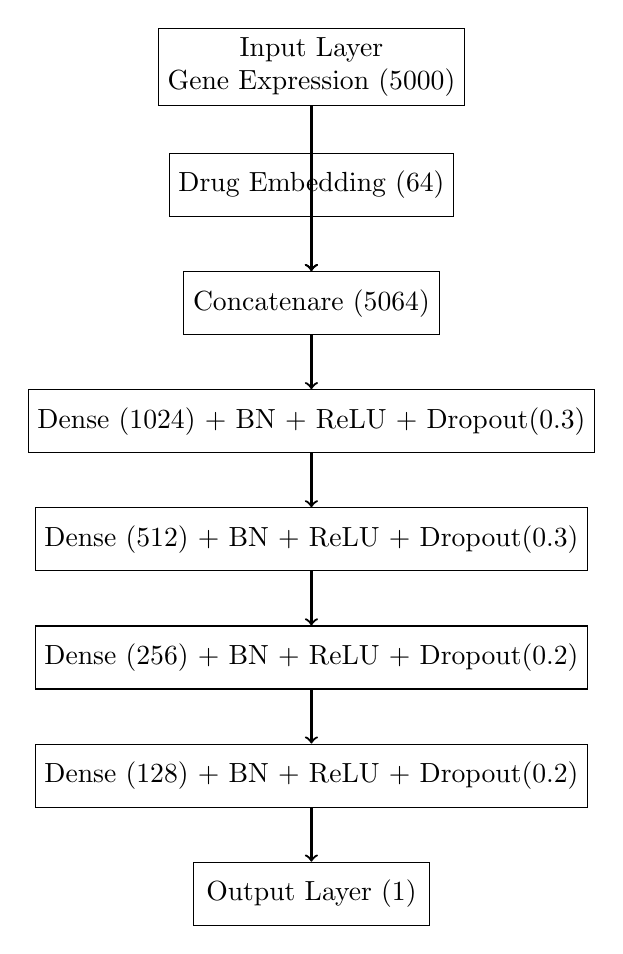
\begin{tikzpicture}[
    layer/.style={rectangle, draw, minimum width=3cm, minimum height=0.8cm, align=center},
    arrow/.style={->, thick}
]
    \node[layer] (input) at (0,0) {Input Layer\\Gene Expression (5000)};
    \node[layer] (embed) at (0,-1.5) {Drug Embedding (64)};
    \node[layer] (concat) at (0,-3) {Concatenare (5064)};
    \node[layer] (fc1) at (0,-4.5) {Dense (1024) + BN + ReLU + Dropout(0.3)};
    \node[layer] (fc2) at (0,-6) {Dense (512) + BN + ReLU + Dropout(0.3)};
    \node[layer] (fc3) at (0,-7.5) {Dense (256) + BN + ReLU + Dropout(0.2)};
    \node[layer] (fc4) at (0,-9) {Dense (128) + BN + ReLU + Dropout(0.2)};
    \node[layer] (output) at (0,-10.5) {Output Layer (1)};

    \draw[arrow] (input) -- (concat);
    \draw[arrow] (embed) -- (concat);
    \draw[arrow] (concat) -- (fc1);
    \draw[arrow] (fc1) -- (fc2);
    \draw[arrow] (fc2) -- (fc3);
    \draw[arrow] (fc3) -- (fc4);
    \draw[arrow] (fc4) -- (output);
\end{tikzpicture}
\caption{Arhitectura rețelei neuronale pentru predicția răspunsului la medicamente}
\label{fig:nn_architecture}
\end{figure}

\subsection{Drug Embeddings}
\label{subsec:drug_embeddings}

În loc de one-hot encoding (vector sparse de dimensiune 200), folosim un \textbf{embedding layer} care învață o reprezentare dense de dimensiune 64 pentru fiecare medicament:

\begin{equation}
\mathbf{e}_d = \text{Embedding}(d) \in \mathbb{R}^{64}
\end{equation}

Această reprezentare permite modelului să învețe similitudini între medicamente. De exemplu, două medicamente cu mecanisme de acțiune similare vor avea embeddings apropiate în spațiul latent.

\subsection{Layere Dense cu Regularizare}
\label{subsec:dense_layers}

Fiecare layer dense aplică următoarea transformare:

\begin{equation}
\mathbf{h}_{l+1} = \text{Dropout}(\text{ReLU}(\text{BatchNorm}(\mathbf{W}_l \mathbf{h}_l + \mathbf{b}_l)))
\end{equation}

unde:
\begin{itemize}
    \item $\mathbf{W}_l, \mathbf{b}_l$ sunt ponderile și bias-urile layer-ului $l$
    \item \textbf{BatchNorm} normalizează activările, stabilizând antrenarea
    \item \textbf{ReLU} este funcția de activare: $\text{ReLU}(x) = \max(0, x)$
    \item \textbf{Dropout} dezactivează aleatoriu o fracție din neuroni în timpul antrenării, prevenind overfitting
\end{itemize}

\subsection{Funcția de Loss}
\label{subsec:loss_function}

Pentru ambele ținte (IC50 și AUC), folosim Mean Squared Error (MSE):

\begin{equation}
\mathcal{L}_{\text{MSE}} = \frac{1}{N} \sum_{i=1}^{N} (y_i - \hat{y}_i)^2
\end{equation}

\subsection{Optimizare}
\label{subsec:optimization}

Utilizăm optimizatorul \textbf{Adam} (Adaptive Moment Estimation) cu:
\begin{itemize}
    \item Learning rate inițial: $\alpha = 0.001$
    \item $\beta_1 = 0.9$, $\beta_2 = 0.999$ (parametrii Adam)
\end{itemize}

Adam combină avantajele momentum-ului cu adaptarea learning rate-ului per parametru, converging mai rapid decât SGD.

\subsection{Learning Rate Scheduling}
\label{subsec:lr_scheduling}

Folosim \textbf{ReduceLROnPlateau} pentru a reduce learning rate-ul când performanța pe validare stagnează:

\begin{itemize}
    \item Dacă loss-ul de validare nu scade timp de 10 epoci, reducem $\alpha \leftarrow \alpha / 10$
    \item Minimum learning rate: $10^{-6}$
\end{itemize}

\subsection{Early Stopping}
\label{subsec:nn_early_stopping}

Antrenarea se oprește dacă loss-ul de validare nu se îmbunătățește după 20 de epoci consecutive. Această strategie:
\begin{itemize}
    \item Previne overfitting
    \item Reduce timpul de antrenare
    \item Returnează modelul cu cea mai bună performanță pe validare
\end{itemize}

\subsection{Hiperparametri}
\label{subsec:nn_params}

Principalii hiperparametri utilizați:

\begin{table}[h]
\centering
\caption{Hiperparametri Rețea Neuronală}
\label{tab:nn_params}
\begin{tabular}{lrl}
\toprule
\textbf{Parametru} & \textbf{Valoare} & \textbf{Descriere} \\
\midrule
drug\_embedding\_dim & 64 & Dimensiunea embedding-urilor \\
hidden\_dims & [1024, 512, 256, 128] & Dimensiunile layerelor ascunse \\
dropout\_rates & [0.3, 0.3, 0.2, 0.2] & Probabilități dropout per layer \\
batch\_size & 128 & Dimensiunea batch-urilor \\
learning\_rate & 0.001 & Learning rate inițial \\
max\_epochs & 200 & Număr maxim de epoci \\
early\_stopping\_patience & 20 & Epoci fără îmbunătățire până la stop \\
\bottomrule
\end{tabular}
\end{table}

\subsection{Avantaje și Dezavantaje}
\label{subsec:nn_pros_cons}

\textbf{Avantaje}:
\begin{itemize}
    \item Flexibilitate: poate învăța relații arbitrar de complexe
    \item Drug embeddings captură similitudini între medicamente
    \item Scalabil la dataset-uri mari (cu GPU)
\end{itemize}

\textbf{Dezavantaje}:
\begin{itemize}
    \item Mai multe hiperparametri de tunat
    \item Necesită mai mult timp de antrenare
    \item Mai puțin interpretabil decât tree-based models
\end{itemize}

\section{Metrici de Evaluare}
\label{sec:metrici}

Pentru a evalua performanța modelelor, folosim următoarele metrici:

\subsection{R² (Coeficient de Determinare)}
\label{subsec:r2}

\begin{equation}
R^2 = 1 - \frac{\sum_{i=1}^{N} (y_i - \hat{y}_i)^2}{\sum_{i=1}^{N} (y_i - \bar{y})^2}
\end{equation}

$R^2$ măsoară proporția de varianță explicată de model. Valori mai mari indică predicții mai bune:
\begin{itemize}
    \item $R^2 = 1$: predicții perfecte
    \item $R^2 = 0$: modelul nu e mai bun decât media
    \item $R^2 < 0$: modelul e mai rău decât media
\end{itemize}

\subsection{RMSE (Root Mean Squared Error)}
\label{subsec:rmse}

\begin{equation}
\text{RMSE} = \sqrt{\frac{1}{N} \sum_{i=1}^{N} (y_i - \hat{y}_i)^2}
\end{equation}

RMSE măsoară eroarea medie de predicție în aceleași unități ca variabila țintă. Valori mai mici sunt mai bune.

\subsection{MAE (Mean Absolute Error)}
\label{subsec:mae}

\begin{equation}
\text{MAE} = \frac{1}{N} \sum_{i=1}^{N} |y_i - \hat{y}_i|
\end{equation}

MAE este mai robustă la outliers decât RMSE.

\subsection{Corelații}
\label{subsec:correlations}

\textbf{Spearman} $\rho$: Corelație bazată pe ranguri (ordinea valorilor). Robustă la relații monotone non-liniare.

\textbf{Pearson} $r$: Corelație liniară. Sensibilă la outliers.

\section{Rezumat}
\label{sec:rezumat_metode}

Am implementat trei metode complementare:

\begin{itemize}
    \item \textbf{Random Forest}: Ensemble de arbori independenți, robust, furnizează feature importance
    \item \textbf{XGBoost}: Gradient boosting cu regularizare, adesea cel mai performant pe date tabulare
    \item \textbf{Rețele Neuronale}: Arhitectură profundă cu drug embeddings, flexibilă și scalabilă
\end{itemize}

Fiecare model are avantaje și dezavantaje, iar compararea lor va revela care abordare este cea mai potrivită pentru predicția răspunsului la medicamente din expresia genică.
